\PassOptionsToPackage{type=CC,modifier=by,version=4.0}{doclicense}
\documentclass[conference,a4paper]{cs-techrep}
\pdfoutput=1 % pdflatex hint for arxiv.org (within first 5 lines)

% Class cs-techrep.cls loads biblatex / biber with predefined options
\addbibresource{embedded.bib}       % its content is declared below, embedded within this tex-file
\addbibresource{webdev_commons.bib} % includes REST, React, Angular, Vue, Svelte, Docker, AWS-*, Socket.IO, and many more!
\addbibresource{cpn_all_all.bib}    % includes all previous CyberLytics@OTH-AW technical reports

% Workaround to make acronym working on current miktex version
% https://tex.stackexchange.com/questions/735500/problem-with-amsmath-cleveref-acronym
\makeatletter
\AtBeginDocument
{
	\def\ltx@label#1{\cref@label{#1}}%add braces
	\def\label@in@display@noarg#1{\cref@old@label@in@display{#1}}%remove braces
	\def\label@in@mmeasure@noarg#1{%
		\begingroup%
		\measuring@false%
		\cref@old@label@in@display{#1}%remove braces for multline, see https://tex.stackexchange.com/q/737204/2388
		\endgroup}%  
} %
\makeatother
% End Workaround


% ======================================================================
% EDIT THESE:

\cstechrepAuthorListTex{Dotzler Martin, Ehrles Andreas, Taach Eduard, Wegerer Nikolas,\\ Weinhut Justin, Christoph P.\ Neumann\,\orcidlink{0000-0002-5936-631X}}
\cstechrepAuthorListBib{Dotzler Martin \& Ehrles Andreas \& Taach Eduard \& Wegerer Nikolas \& Weinhut Justin \& Christoph P. Neumann}

% Capitalization: https://capitalizemytitle.com/style/Chicago/
\cstechrepTitleTex{GetraenkeIO: Eine Getränkelagerverwaltung mit Bestandsstatistik für Vereinsheime}
 % IF you need manual linebreaks in the titel, then clone the title without linebreaks for BibTeX:
\cstechrepTitleBib{{\cstechrepTitleTex}}

%\cstechrepDepartment{CyberLytics\-/Lab at the Department of Electrical Engineering, Media, and Computer Science}
\cstechrepDepartment{CyberLytics\-/Lab an der Fakultät Elektrotechnik, Medien und Informatik} % DE
\cstechrepInstitution{Ostbayerische Technische Hochschule Amberg\-/Weiden}
%\cstechrepAddress{Amberg, Germany}
\cstechrepAddress{Amberg, Deutschland} % DE
%\cstechrepType{Technical Report}
\cstechrepType{Technischer Bericht} % DE
\cstechrepYear{2025}
\cstechrepMonth{7}
\cstechrepNumber{CL-TR-\cstechrepYear{}-42}
%\cstechrepLang{english}  % en-US
\cstechrepLang{ngerman} % DE

% Special remark on babel/csquotes terminology in regard with US-vs-UK:
% en-US  = [english]/[american]/[usenglish] (+ [canadian])
% en-UK  =           [british] /[ukenglish] (+ [australian]) <OXFORD>
% For cs-techrep (like ACM), the recommended english variant is en-US!

% DO NOT DELETE THIS:
\filecontentsForceExpansion|[] % force command expansion inside a filecontents* environment
\begin{filecontents*}[overwrite]{selfref.bib}
    @TECHREPORT{selfref,
        author = {|cstechrepAuthorListBib},
        title  = {\cstechrepTitleBib},
        institution = {\cstechrepInstitution, \cstechrepDepartment},
        type   = {\cstechrepType},
        number = {\cstechrepNumber},
        year   = {|cstechrepYear},
        month  = {|cstechrepMonth},
        langid  = {|cstechrepLang},
    }
\end{filecontents*}

% ======================================================================
% EDIT THIS:

\begin{filecontents}[overwrite]{embedded.bib}
@Online{conatiners,
    author = {IBM},
    title = {Was sind Container?},
    url = {https://www.ibm.com/de-de/topics/containers},
    year = {2025}
}
@Online{sqlmodel,
    author = {Sebastián Ramírez},
    title = {SQLModel},
    url = {https://sqlmodel.tiangolo.com/},
    year= {2025}
}
@Online{openapi,
    author = {The Linux Foundation},
    title = {OpenAPI-Spezifikation},
    url = {https://spec.openapis.org/oas/latest.html},
    year= {2025}
}
@Online{swagger,
    author = {{SMARTBEAR}},
    title = {Swagger},
    url = {https://swagger.io/},
    year= {2025}
}

@online{ieee2015howto,
    author = {Michael Shell},
    title = {How to Use the {IEEEtran} \LaTeX\ Class},
    url = {http://mirrors.ctan.org/macros/latex/contrib/IEEEtran/IEEEtran_HOWTO.pdf},
    year = {2015}
}
@online{ieee2018formattingrules,
    author = {{IEEE}},
    title = {Conference Template and Formatting Specifications},
    url = {https://www.ieee.org/content/dam/ieee-org/ieee/web/org/conferences/Conference-template-A4.doc},
    year = {2018}
}
@online{iaria2014formattingrules,
    author = {{IARIA}},
    title = {Formatting Rules},
    url = {http://www.iaria.org/formatting.doc},
    year = {2014}
}
@online{iaria2009editorialrules,
    _author = {Cosmin Dini},
    author = {{IARIA}},
    title = {Editorial Rules},
    url = {https://www.iaria.org/editorialrules.html},
    year = {2009}
}
@online{languagetool,
    author = {{LanguageTooler GmbH}},
    title  = {{LangueTool}},
    url    = {https://languagetool.org/overleaf}
}
@online{overleaf,
    author = {{Digital Science UK Limited}},
    title  = {{Overleaf}},
    url    = {https://www.overleaf.com}
}
@online{drinkscounter,
    author = {{Matthias Aigner}},
    title = {{Getränke Zähler App}},
    url = {https://drinkscounter.com/de/getraenke-zaehler-app.html}
}
@online{getraenkelisteapp,
    author = {{iqmeta GmbH}},
    title = {{Getränkeliste App}},
    url = {https://iqmeta.com/gliste/}
}
@online{getraenkewart,
    author = {{sparse creations GmbH}},
    title = {{Getränkewart 2.0}},
    url = {https://getraenkewart.com/}
}
\end{filecontents}

\usepackage{fontawesome} % i.a., \faWarning{}
\usepackage{relsize}     % i.a., \textsmaller{...}
\usepackage{lipsum}      % for blindtext
\usepackage{enumitem}
% ======================================================================

% cf. https://ctan.org/pkg/acronym
% Usage:
% singular, within sentence       = \ac{gui}
% singular, beginning of sentence = \Ac{gui}
% plural, within sentence         = \acp{gui}
% plural, beginning of sentence   = \Acp{gui}
\begin{acronym}
    \acro{gui}[GUI]{Graphical User Interface}
    \acro{ide}[IDE]{Integrated Development Environment}
    \acro{orm}[ORM]{Object-Relational Mapping}
    \acro{cors}[CORS]{Cross-Origin Resource Sharing}
    \acro{crud}[CRUD]{Create, Read, Update und Delete}
\end{acronym}

% https://www.silbentrennung24.de/
% https://www.hyphenation24.com/
\hyphenation{block-chain block-chains Ethe-re-um}

\begin{document}
\selectlanguage{\cstechrepLang}

\maketitle

\begin{abstract}
GetraenkeIO ist eine webbasierte Software zur Verwaltung des Getränkelagers in Vereinen oder anderen Einrichtungen. Sie ermöglicht es registrierten Benutzern, Getränke eigenständig zu buchen, während Administratoren mit erweiterten Rechten Zugriff auf Bestandsstatistiken und Verwaltungsfunktionen haben. Das System unterstützt die effiziente Verwaltung des Lagers.

Technologisch basiert die Anwendung auf einem Python-Backend, das über eine REST-API mit einem React-basierten Frontend kommuniziert. Die Lagerbestände und andere relevante Daten werden in einer relationalen PostgreSQL-Datenbank gespeichert. Docker wird verwendet, um die Anwendung flexibel bereitzustellen und eine einfache Skalierbarkeit zu gewährleisten.
\end{abstract}

% A list of IEEE Computer Society appoved keywords can be obtained at
% http://www.computer.org/mc/keywords/keywords.htm
\begin{IEEEkeywords}
Docker, React, TypeScript, Python, PostgreSQL, Container, Cloud
\end{IEEEkeywords}

\section{Einleitung und Projektziele}
In vielen Vereinsheimen stellt die Getränkeverwaltung nach wie vor eine organisatorische Herausforderung dar. Die Ausgabe und Bezahlung erfolgen häufig auf Vertrauensbasis, wodurch es schwierig ist, den Überblick über Lagerbestände und Einnahmen zu behalten. Auch gängige Hilfsmittel wie Strichlisten oder Excel-Tabellen sind fehleranfällig und erfordern eine regelmäßige, manuelle Pflege.

GetraenkeIO bietet hierfür eine digitale und einfach bedienbare Lösung. Die webbasierte Anwendung stellt eine benutzerfreundliche Oberfläche bereit, über die Vereinsmitglieder selbstständig Getränke auswählen und ihre Käufe erfassen können. Im Hintergrund verwaltet das System automatisch den Lagerbestand, dokumentiert Zahlungen und erstellt grundlegende Statistiken.

Verantwortliche erhalten so einen klaren Überblick über Bestände und Konsumverhalten, während die alltägliche Verwaltung spürbar vereinfacht wird. Als besonderes Merkmal integriert GetraenkeIO alle relevanten Funktionen in einer kompakten Anwendung, die speziell auf den Einsatz in kleinen Organisationen zugeschnitten ist.

\section{Verwandte Arbeiten}
Die Verwaltung von Getränken ist in vielen Vereinen eine notwendige Aufgabe. Daher ist es nicht verwunderlich, dass es für eine leichtere Handhabung dieses Vorgangs bereits bestehende Anwendungen gibt, welche eine Vereinfachung versprechen. Bei diesem Vergleich interessieren uns vor allem die Unterschiede, insbesondere jene im Bereich der Monetarisierung.
Alle drei hier betrachteten Anwendungen basieren auf einer teilweise zahlungspflichtigen Strategie. So ist es bei der Getränke Zähler App \cite{drinkscounter}, der Getränkeliste App \cite{getraenkelisteapp} und dem Getränkewart 2.0 \cite{getraenkewart} jeweils möglich je nach Anbieter mit bis zu 3 bis 10 Nutzern die Anwendung jeweils kostenlos zu nutzen. Sollte die App jedoch von mehr Benutzern verwendet werden, so werden jeweils monatliche oder jährliche Kosten für die Nutzung fällig. Dies ist ein großer Unterschied zu GetraenkeIO, da diese nicht nur kostenfrei nutzbar ist, sondern dank der MIT Lizenz sogar Open Source. Im Gegenteil zu den drei anderen genannten Lösungen ist es bei GetraenkeIO deshalb ebenfalls möglich die Software auf eigener Hardware laufen zu lassen und so die komplette Kontrolle über die eigenen Daten zu erhalten.

\section{Architekturziele} % \textbar{} \textquote{Architekturziele}}
\subsection{Kontextabgrenzung}
Das System zur Getränkeverwaltung in Vereinsheimen soll von folgenden Nutzern genutzt werden:
\begin{enumerate}
	\item \textbf{Benutzer}: 
	Der reguläre Benutzer des Systems, der in einem Vereinsheim o.ä. ab und zu ein Getränk trinkt und dieses im System buchen möchte, damit er seine Zeche bezahlen kann.
	\item \textbf{Admin}: 
	(Auch Getränkewart) des Vereinsheims, der sich um den Getränkenachschub kümmert und regelmäßig das Geld für die Getränke kassiert.
\end{enumerate}
Den Benutzern des Systems wird eine Web-Oberfläche zur Interaktion bereitgestellt, die folgende Funktionalität bietet.\\
\textbf{Benutzer} können:
\begin{itemize}
	\item sich registrieren und einloggen.
	\item eine Übersicht über alle verfügbaren Getränke anzeigen.
	\item ein bestimmtes Getränk buchen.
	\item ihren Getränkeverlauf einsehen.
\end{itemize}
\textbf{Admins} können alles was der Benutzer kann und zusätzlich:
\begin{itemize}
	\item Guthaben von Benutzern aufladen.
	\item Getränkedaten (Bestand, Preis, verfügbare Getränke,...) verwalten.
	\item Statistiken über den Getränkeverbrauch einsehen.
\end{itemize}
\textbf{Nicht} Teil des Systems sind: 
\begin{itemize}
	\item Funktionalität zur Beschaffung von Getränken.
	\item Verwaltung des tatsächlichen Kassenstandes.
\end{itemize}
\subsection{Rahmenbedingungen}
\begin{itemize}
	\item Zum Betreiben des Systems muss eine \textbf{Internetverbindung} bestehen.
	\item Es gibt nur \textbf{einen Administrator} pro installiertem System, dessen Passwort bei der Installation gesetzt wird.
\end{itemize}
\subsection{Architekturstil}
Als Architekturstil für die Applikation wurde eine dreischichtige Architektur bestehend aus:
\begin{itemize}
	\item \textbf{Frontend}: React Web-App
	\item \textbf{Backend}: Python REST-API
	\item \textbf{Datenbank}: Relationale PostgreSQL Datenbank
\end{itemize}
gewählt.
%Provides
%(1) a visualization of the external systems and users with which the system interacts (\textquote{Kontextabgrenzung}),
%(2) the most important technical and organizational preconditions (\textquote{Rahmenbedingungen}),
%(3) quality/non-functional requirements (\textquote{Qualitätsziele}), and/or
%(4) architectural style design decisions with formative patterns of the solution (\textquote{Architekturstil})
%as well as (5) the applied programming language(s).

\section{Architektur von GetraenkeIO} %of CatchyName \textbar{} Results \textbar{} Structural Design \textbar{} \textquote{Bausteinsicht}

\subsection{Technologie-Stack} % \textbar{} Overall System \textbar{} \textquote{Gesamtsystem}}
Die GetraenkeIO-Anwendung besteht aus einer dreischichtigen Architektur aus Frontend, Backend und Datenhaltungsschicht.
Jede Schicht soll von den anderen abgegrenzt in einem eigenen Container \cite{conatiners} laufen.
Das Frontend besteht aus einer React-Anwendung \cite{react}.
Als Backend wird eine Python-Anwendung \cite{python} verwendet.
Diese benutzt das Web-Framework FastAPI \cite{fastapi} und stellt damit dem Frontend eine RESTful-Schnittstelle \cite{restful} zum Datenaustausch zur Verfügung.
Zur Datenhaltung wird die relationale Datenbank PostgreSQL \cite{postgresql} genutzt.
Die Kommunikation zwischen Datenbank und Backend übernimmt das Framework SQLModel \cite{sqlmodel}, welches mittels \ac{orm} die Datenbanktabellen als Python-Objekte zur Verfügung stellt. In \autoref{fig:bausteinsicht-architektur} werden die Architekturbausteine und deren Beziehungen grafisch dargestellt.

\begin{figure}[h]
	\centering
	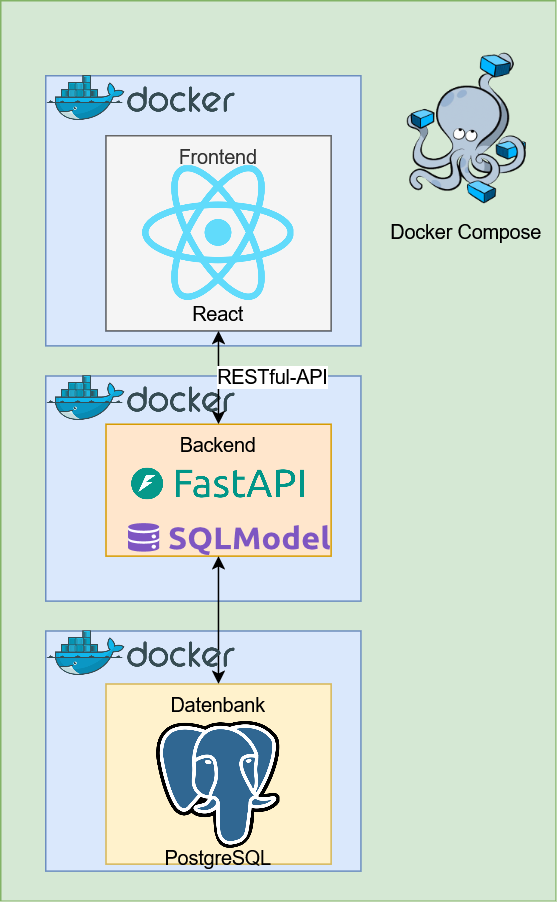
\includegraphics[width=0.9\linewidth]{Bausteinsicht-Architektur.drawio}
	\caption{Bausteinsicht über den Technologie-Stack und die verwendeten Technologien und deren Zusammenspiel.}
	\label{fig:bausteinsicht-architektur}
\end{figure}


%\subsubsection{Vorlage Hr. Neumann}
%Provides
%(1) design decisions based on the previously defined requirements and
%(2) a visualization of the functional structure at top level including relationships (\textquote{Grobe Zerlegung}), thus, gives an overview on modules, frameworks, and middleware.
%
%In discussions of multi-tier architecture, layer is often used interchangeably -- and mistakenly -- for tier. They aren't the same. A \textquote{layer} refers to a functional division of the software, but a \textquote{tier} refers to a functional division of the software that runs on infrastructure separate from the other divisions. The Contacts app on your phone, for example, is a three-layer application, but a single-tier application, because all three layers run on your phone.
%
%In discussions concerning multi-tier architecture, the term \textquote{layer} is frequently misused interchangeably with \textquote{tier}, despite their distinct meanings. A layer denotes a functional partition within the software, whereas a tier signifies a functional division that operates on separate infrastructure from other divisions/tiers. For instance, the Camera app or Settings app on your phone exemplifies a three-layer application but remains a single-tier application since all three layers run on your phone.


\subsection{Frontend}
Das Frontend der Anwendung wurde mit dem Framework \textbf{React} umgesetzt. Zusammen mit dem Tool \textbf{Vite} wird eine schnelle Projektinitialisierung als auch ein sehr performantes Hot Module Replacement bereitgestellt. Dadurch können Änderungen am Code durch einfaches Speichern in Echtzeit im Browser dargestellt werden. Dies führt zu einer deutlich angenehmeren und zeiteffizienteren Entwicklung. \newline
Als Programmiersprache wurde \textbf{TypeScript} gewählt. Im Vergleich zu JavaScript bietet TypeScript eine statische Typisierung von Variablen, Funktionen und anderen Komponenten. Dies ermöglicht eine frühzeitige Fehlererkennung - was sich positiv auf die Entwicklungszeit auswirkt - als auch bessere Lesbarkeit des Codes und vereinfachte Wartungen bei größeren und komplexeren Projekten. \newline
Für die bessere Gestaltung der Benutzeroberfläche wird \textbf{Inline-CSS} in den React-Komponenten verwendet. Das heißt CSS-Stile liegen nicht in eigenen Dateien sondern werden mithilfe der \texttt{style=\{\{\}\}}-Syntax direkt im JSX/TSX-Code eingebunden. Auf separate Dateien und externe Styling-Frameworks wie \textbf{TailwindCSS} wurde bewusst verzichtet, um die Syntax möglichst komponentennah und unkompliziert zu halten.	\newline
Die Kommunikation mit dem Backend erfolgt ausschließlich über eine Rest-API. Hierfür wird die Bibliothek \textbf{Axios} verwendet. Diese bietet eine einfache Anbindung an diverse Endpunkte. Die empfangenen Daten liegen im JSON-Format vor und werden von den einzelnen Komponenten individuell verarbeitet und angezeigt. \newline
Für die zentrale Zustandsverwaltung wird die Bibliothek \textbf{Redux} verwendet. Dadurch lassen sich globale Zustände und Daten einfach effizient verwalten. Im Falle des Logins bzw. der Registierung sorgt ein globaler Zustand dafür, dass nicht eingeloggte Benutzer keinen Zugriff auf geschützte Routen haben, um unerlaubten Zugriff zu vermeiden. Die Nutzerrrollen des angemeldeten Users werden auf die gleiche Art und Weise gespeichert. So hat der Nutzer zudem nur Zugriff auf die für seine Rolle vorgesehenen Seiten und Funktionen. Die Integration erfolgt mithilfe des \textbf{react-redux}-Bindings, wodurch der State über das gesamte Frontend hinweg einheitlich zugänglich ist.\newline
\autoref{fig:oberflaechegetraenkeuebersicht} zeigt die Getränkeübersichtsseite des Frontends.

\begin{figure*}[h]
	\centering
	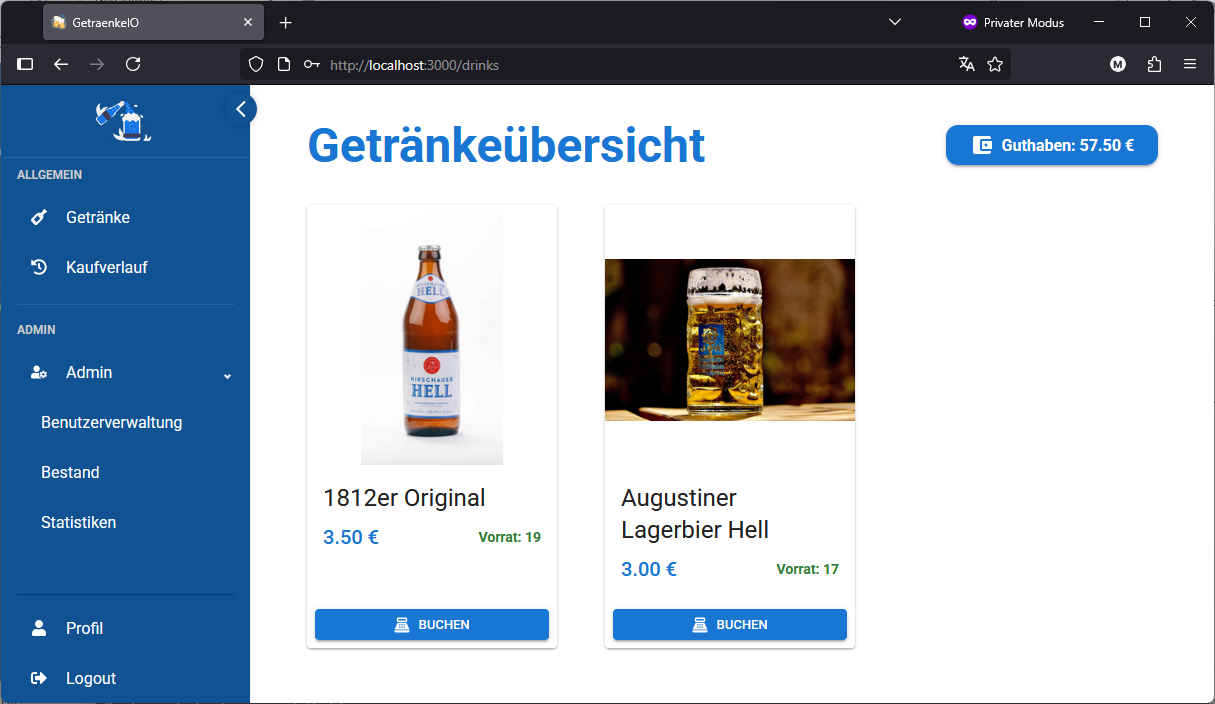
\includegraphics[width=1.0\linewidth]{Oberflaeche_Getraenkeuebersicht}
	\caption{Zentrale Seite mit Getränkeübersicht, Guthabenanzeige und der Möglichkeit ein Getränk zu buchen.
	Aktuell ist ein Admin eingeloggt, daher sind links in der Sidebar auch die Menüs für den Admin sichtbar.}
	\label{fig:oberflaechegetraenkeuebersicht}
\end{figure*}


\subsubsection{Struktur und Komponenten}
Der Sourcecode ist in verschiedene Ordner unterteilt. Zusammengehörige Funktionalitäten sind dabei gruppiert, um die Wartbarkeit zu verbessern. Im Folgenden werden die wichtigsten Ordner / Dateien und deren Aufgaben beschrieben.

\begin{description}
	\item[src/api] Enthält die zentrale \texttt{axiosInstance} über welche alle Http-Requests abgewickelt werden.
	\item[src/components] Beinhaltet wiederverwendbare UI-Komponenten, z. B.: \texttt{AuthSidebar} \texttt{HomeSidebar} und \texttt{ProtectedLayout}.
	\item [src/features] Redux-Slices zur Authentifizierung sowie Methoden, die verschiedenen API-Calls ausführen.
	\item [src/models] Definiert gemeinsame TypeScript-Interfaces, die über die ganze Anwendung hinweg verwendet werden.
	\item [src/pages] Eigenständige Seiten wie \texttt{Login} und \texttt{Register}, die unabhängig vom Layout (ohne Sidebar) fungieren.
	\item[src/store] Konfiguration des zentralen Redux-Stores für das globale State-Management.
	\item[src/views] Seiten, die nach dem Einloggen angezeigt werden können und das \texttt{ProtectedLayout} sowie die \texttt{HomeSidebar} verwenden.
	\item[src/App.tsx] Hauptkomponente der Anwendung. Hier wird das grundlegende Routing sowie das globale Layout (z.\,B. Sidebar, Protected Routes) definiert.
	\item[src/main.tsx] Einstiegspunkt der React-App. Hier wird der Redux-Provider eingerichtet und die Anwendung in das DOM eingebunden.
\end{description}

\subsection{Backend} % Application Tier \textbar{} \textbar{} \textquote{Anwendungskern} 
Das Backend von GetraenkeIO ist als Python Applikation geschrieben.
Mithilfe der Frameworks FastAPI wird eine REST-API für das Frontend zur Verfügung gestellt. \\  
FastAPI ist ein Framework, das speziell zum Entwickeln von REST-APIs erstellt wurde und sehr intuitiv zu bedienen ist.
Es ist damit möglich mit relativ wenigen Zeilen Code einen funktionierenden Endpunkt, inklusive Validierung der Werte zu erzeugen. Ebenfalls unterstützt es verschiedene Middlewares. Konkret wurde die CORS-Middleware genutzt. Diese ermöglicht es \ac{cors} Anfragen vom Frontend entgegenzunehmen.
Eine Besonderheit von FastAPI ist, dass eine API-Dokumentation in Form eines OpenAPI-Dokuments \cite{openapi} automatisiert erstellt wird. Diese wird auf der Route \emph{/docs} als interaktive Oberfläche mittels SwaggerUI  \cite{swagger} zur Verfügung gestellt. Dies erleichtert die Abstimmung zwischen den Entwicklerteams von Front-und Backend. \\  
Für die Verwaltung der Datenbankverbindung wurde das Framework SQLModel gewählt. Dieses wurde vom gleichen Entwickler wie FastAPI entwickelt. Deshalb ist eine Integration dieser beiden Technologien sehr gut möglich. SQLModel ist ein \ac{orm}-Framework.
Das Datenmodell für die Datenbank wird von SQLModel auf Basis von den im Python-Code erzeugten Datenklassen (Models) erstellt. Ebenfalls müssen für die gängigen \ac{crud} Operationen keine direkten SQL-Abfragen erzeugt werden, es genügt das zugehörige Model  zu ändern und an die Datenbanksession weiterzugeben.

\subsubsection{Struktur und Komponenten}
Der Quellcode der Backend-App gliedert sich in mehrere Komponenten (Ordner/Dateien), deren Funktion im Folgenden erklärt wird.
\begin{description}[style=standard]
	\item[app/api/routes] Logik für alle Routen, der REST-Schnittstelle.
	\item[app/api/dependencies.py] Funktionen/Abhängigkeiten, welche von mehreren Endpunkt-Implementierungen aus \emph{app/api/routes} verwendet werden (Benutzer-Authentifizierung, Zugriff auf Datenbank-Session, Überprüfung ob aktueller Benutzer Admin-Rechte hat).
	\item[app/core] Sämtliche Logik zur Konfiguration der Anwendung (Datenbank, Passwort-Hash-Funktion, Lesen der Einstellungen aus Umgebungsvariablen).
	\item[app/crud] Logik zur Interaktion mit der Datenbank (Erstellen, Lesen, Schreiben und Löschen von den Datenmodellen aus \emph{/app/models}).
	\item[app/models] Datenmodelle für die in der Datenbank  gespeicherten Daten. Ebenfalls die zugehörigen Datenmodelle, die in den Endpunkten (GET/POST) verwendet werden und die Logik zum validieren der Daten.
	\item[app/tests] Komponenten-Tests für die Anwendung, welche mithilfe von pytest \cite{pytest} automatisch bei einem \emph{push} ins Git-Repository ausgeführt werden.
	\item[main.py] Initialisierung und Start-Up der Anwendung.
	\item[requirements.txt] Enthält alle genutzten Pakete, um diese automatisiert installieren zu können.
	\item[.env.example] Beispielhafte .env-Datei, welche die zur Konfiguration nutzbaren Umgebungsvariablen und Beispielwerte für diese enthält.
\end{description}

\subsubsection{REST-Schnittstelle}
Die einzige Schnittstelle zwischen Front-und Backend ist die REST-Schnittstelle. Diese stellt alle relevanten Daten und Informationen für das Frontend im JSON-Format bereit. Im folgenden werden alle wichtigen Endpunkte genauer beschrieben:


\begin{description}[style=standard]
	\item[GET /users] Gibt eine Liste mit Details über alle Benutzer zurück.
	Ist nur für den Admin nutzbar.
	\item[GET /users/me] Gibt Informationen über den aktuell eingeloggten Benutzer zurück.
	\item[GET /users/\{user\_name\}] Gibt Informationen über den Benutzer mit dem Name \emph{user\_name} zurück.
	Ist nur für den Admin nutzbar.
	\item[POST /users/] Endpunkt zum Erstellen eines neuen Benutzers bei seiner Registrierung.
	\item[POST /users/\{user\_id\}/recharges] Endpunkt zum Aufladen des Guthabens eines Benutzers.
	Ist nur für den Admin nutzbar.
	\item[GET /users/\{user\_id\}/recharges] Gibt alle Aufladungen eines Benutzers zurück.
	Ist für den Benutzer selbst und den Admin benutzbar.
	\item[GET /drinks] Gibt eine Liste mit allen Daten der aktuell vorhandenen Getränke zurück.
	\item[GET /drinks/\{drink\_id\}] Gibt das Getränk mit der angegebenen Getränke-ID zurück.
	\item[POST /drinks] Erlaubt es dem Admin ein neues Produkt zu erstellen. Dazu müssen alle Attribute des neuen Getränks in einem JSON-Objekt mitgegeben werden. Ausgenommen davon ist die ID, welche bei der Erstellung des Eintrags in der Getränketabelle automatisch mithilfe eines UUID-Generators erstellt wird.
	\item[PUT /drinks/\{drink\_id\}]Lässt Administratoren die Attribute der Getränke ändern. Dabei können beliebige Kombinationen an Attributen eines Getränks gleichzeitig geändert werden. Lediglich die ID ist hierüber nicht veränderbar. Zum ändern der gewünschten Attribute werden diese Entsprechend mit neuen Werten als JSON-Objekt an die API übergeben. Ist ein Attribut nicht im Objekt vorhanden, so bleibt dort der Ursprüngliche Wert erhalten.
	\item[DELETE /drinks/\{drink\_id\}] Lässt Administratoren ein Getränk löschen. Dabei wird dem Nutzer nach erfolgreicher Löschung eine Kopie des Objekts zurückgegeben.
	\item[POST /transactions] Ermöglicht es Nutzern ein Getränk zu kaufen. Dabei wird das Guthaben des Nutzers um den Gesamtpreis verringert und die Stückzahl des Getränks entsprechend angepasst. Zudem wird die Transaktion in einer separaten Tabelle protokolliert.
	\item[GET /transactions] Gibt einem Admin alle getätigten Transaktionen als Liste zurück.
	\item[GET /transactions/me] Gibt Nutzern alle von ihnen durchgeführte Transaktionen als Liste zurück.
\end{description}

\subsection{Datenhaltung} % Data Tier \textbar{} Persistence
Zur Datenhaltung in der Produktionsumgebung wird eine relationale PostgreSQL-Datenbank verwendet. 
Die Kommunikation mit dieser findet über das SQLModel-Framework statt. 
Da ein \ac{orm}-Framework verwendet wird, könnte die Datenbank relativ einfach gegen alle anderen von diesem Framework unterstützen Datenbanken ausgetauscht werden. 
In der Anfangsphase der Entwicklung wurde diese Möglichkeit genutzt, um SQLite \cite{sqlite} als Entwicklungsdatenbank verwenden zu können und durch die einfache Konfiguration schnell ein lauffähiges System erzeugen zu können.
\begin{figure}[h]
	\centering
	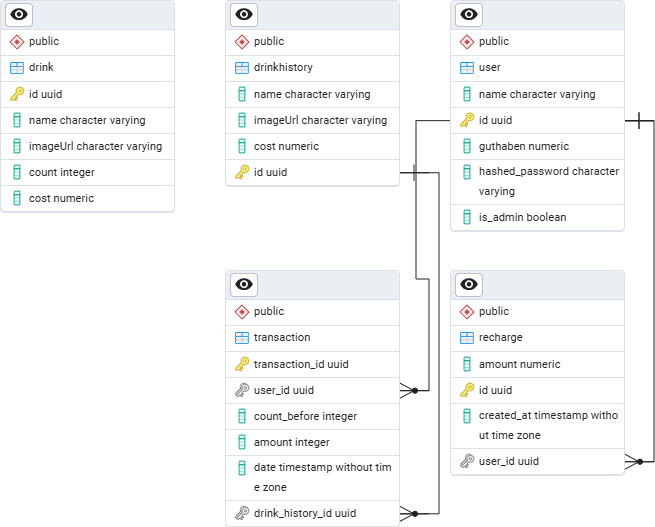
\includegraphics[width=0.9\linewidth]{database_erd}
	\caption{ER-Diagramm zur PostgreSQL Datenbank}
	\label{fig:erd-modell-datenbank}
\end{figure}

Die Daten der Getränkeverwaltung werden in unserer Datenbank, wie in Abbildung \ref{fig:erd-modell-datenbank} beschrieben, auf fünf verschiedene Tabellen aufgeteilt. So werden aktuelle Nutzer und Getränke in jeweils einzelnen Tabellen abgespeichert. Abseits davon sind die weiteren Tabellen zur Überwachung der getätigten Aktionen verantwortlich. Somit wird das Aufladen von Guthaben in der recharge Tabelle und jeder Kauf in der transaction Tabelle abgespeichert. Um jedoch sowohl die ursprünglichen Preise, als auch weitere möglicherweise veränderte Attribute der Getränke für spätere Analysezwecke korrekt vorliegen zu haben, wird für jedes veränderte Getränk, das gekauft wird, ebenfalls ein Eintrag in der drinkhistory Tabelle erstellt.

%\subsection{Optional: Infrastructure and Deployment \textbar{} Distribution Perspective \textbar{} \textquote{Verteilungssicht}}
%Provides (1) information about configuration, exact software versions, SBOM, DevOps, Cloud, AWS, and others.
%Should add (2) security-related considerations or disclaimers.
%Could include (3) a software bill of materials (SBOM), at least for the major libraries or frameworks.


\section{Herausforderungen \& Probleme}

Im Laufe der Entwicklung unseres Projekts sind uns einige Probleme und Herausforderungen begegnet, aus denen wir lernen konnten.

\subsection*{1. Authentifizierungsfehler bei API-Anfragen}

Ein technisches Problem war, dass die Getränke aus dem Backend nicht geladen wurden. Grund dafür war, dass die Anfragen teilweise ohne Authentifizierung abgeschickt wurden. Das lag daran, dass verschiedene HTTP-Bibliotheken verwendet wurden (einmal Axios, einmal fetch), und nicht immer die richtigen Zugangsdaten mitgesendet wurden. Nachdem wir das mit dem jeweiligen Teammitglied besprochen haben, wurde der Fehler schnell behoben.

\subsection*{2. Fehlermeldungen beim Erstellen des Frontend-Docker-Containers}

Beim Docker-Build des Frontends sind wir auf Probleme gestoßen, weil der TypeScript-Compiler auf ungenutzte Importe gestoßen ist. Diese waren im Code zwar nicht relevant, haben aber den Buildprozess gestört. Nachdem diese Importe bereinigt wurden, konnte das Frontend erfolgreich als Container gebaut werden.

\subsection*{3. Zugriffsrechte im Frontend nicht korrekt umgesetzt}

Ein weiterer Fehler betraf die Zugriffsbeschränkung für Admin-Funktionen. Es war möglich, auch ohne Admin-Rechte gewisse Admin-Routen im Frontend aufzurufen, solange man eingeloggt war. Das wurde intern schnell erkannt und korrigiert.

\subsection*{4. CORS-Konfiguration unvollständig}

Bei der Kommunikation zwischen Frontend und Backend kam es zu Problemen mit CORS (Cross-Origin Resource Sharing). Eine benötigte Origin war nicht in der Konfiguration des Servers freigegeben, was zu abgelehnten Anfragen führte. Dieser Fehler wurde durch Ergänzen der fehlenden Origin behoben.


\section{Fazit und Ausblick} % Conclusion and Future Work \textbar{} \\ \textquote{Fazit und Ausblick}

Wir haben für unser Empfinden eine gute Lösung für eine webbasierte Getränkeverwaltung für Vereine oder auch andere Einrichtungen geschaffen. Unsere gesteckten Ziele wurden weitestgehend erreicht. Sowohl unsere \emph{Muss-} als auch \emph{Soll-Anforderungen} wurden vollumfänglich erfüllt. Die traditionellen Probleme der manuellen Verwaltung durch Strichlisten und Excel-Tabellen werden hierbei durch unser System abgelöst und bieten stattdessen eine automatisierte digitale Lösung.

Ein Hauptaugenmerk bei unserem Projekt lag auf der Benutzerfreundlichkeit. Vereinsmitglieder können ohne administrative Unterstützung eigenständig Getränke buchen. Administratoren erhalten dagegen einen umfangreichen Überblick über Getränkebestände, Konsumverhalten und Umsatz durch das integrierte Statistik- und Verwaltungssystem. Die von uns gewählte dreischichtige Architektur mit React im Frontend, FastAPI im Backend und einer PostgreSQL-Datenbank hat sich als robust und skalierbar erwiesen.

Eine Möglichkeit, \textit{GetraenkeIO} weiter zu optimieren, wäre die Integration von Zahlungsdienstleistern wie PayPal, die eine automatisierte Guthabenaufladung ermöglichen würde. Benutzer könnten ihr Guthaben selbstständig ohne Adminunterstützung aufladen. Dies würde den Verwaltungsaufwand für Administratoren deutlich reduzieren und die Kassenlage des Vereins oder der Einrichtung verbessern, da Zahlungen direkt in Echtzeit eingingen.


%%% Previous TechReps
%\nocite{ModA-TR-2023SS-WAE-TeamWeiss-Neunerln}
%\nocite{ModA-TR-2023SS-BDCC-TeamRot-CompVisPipeline}
%\nocite{ModA-TR-2023SS-BDCC-TeamBlau-NauticalNonsense}
%\nocite{ModA-TR-2023SS-BCN-TeamGruen-TorpedoTactics}
%\nocite{ModA-TR-2023SS-BCN-TeamCyan-Stockbird}
%\nocite{ModA-TR-2023SS-BCN-TeamBlau-FancyChess}
%\nocite{ModA-TR-2023WS-SWT-TeamRot-SGDb}
%\nocite{ModA-TR-2023WS-SWT-TeamGruen-OPCUANetzwerk}
%\nocite{ModA-TR-2022SS-WAE-TeamWeiss-WoIstMeinGeld}
%\nocite{ModA-TR-2022SS-BDCC-TeamWeiss-TwitterDash}
%\nocite{ModA-TR-2022SS-BDCC-TeamRot-Reddiment}
%\nocite{ModA-TR-2022SS-BDCC-TeamGruen-ExplosionGuy}
%\nocite{ModA-TR-2022SS-BDCC-TeamCyan-OTHWiki}
%\nocite{ModA-TR-2022WS-SWT-TeamGruen-Graphvio}
%\nocite{ModA-TR-2021SS-WAE-TeamWeiss-CovidDashboard}
%\nocite{ModA-TR-2021SS-WAE-TeamRot-FireForceDefense}
%\nocite{ModA-TR-2021SS-WAE-TeamGruen-MedPlanner}

% ======== References =========
\sloppy
\printbibliography[notcategory=selfref]

\end{document}
